\section{The Slack Principle}\label{sec:slack}

\Cref{lem:bidding} and \cref{prop:master} price the chokepoint when Europe's exit premium is positive. On our reading of the record since 2019 (\cref{sec:evidence}), it has not been, and Washington has still asked Europe for a great deal. This section asks how much a patron can obtain from an ally whose premium is negative. The answer is the ally's slack, $\Lambda=\pos{-Q}$, plus whatever the patron can threaten that does not depend on the ally's alignment. The idea that a coercer's power lies in the slack of the target's participation constraint belongs to \citet{clayton2026putting} and \citet{clayton2026framework}. We extend it to threats that cut off an ally for whom a rival is bidding.

\subsection{Bite, budgets and assurance}\label{sec:slackprinciple}

Consider one period in which Europe is aligned, its premium is $Q$, and it receives $\pos{Q}$ from the bidding stage. Washington has a finite set of demands. Demand $k$ costs Europe $t_k>0$ and is worth $w_k>0$ to the United States. A concession is \emph{reversible} if exit would undo it, so that it lowers Europe's aligned payoff and leaves its exit payoff unchanged. Policy alignment is of this kind. A limit on servicing Chinese fabs is reversible, because a Europe that exited would resume servicing; so are tariff cuts and export-control rules. A concession is \emph{sunk} if it lowers both payoffs: payments, purchases, and transfers of assets or of control over them.

Washington backs its demands with instruments (\cref{sec:security}). Withdrawing a set $J$ of instruments from an aligned Europe for the period lowers Europe's aligned payoff by $\Delta^A(J)$ and its exit payoff by $\Delta^X(J)$, with $0\le\Delta^X(J)\le\Delta^A(J)$ and both nondecreasing in $J$. We call
\[
u(J)=\Delta^X(J)\qquad\text{and}\qquad d(J)=\Delta^A(J)-\Delta^X(J)
\]
the unconditional and conditional parts of $J$. The conditional part is what Europe would lose by exiting anyway; for a single instrument it is the $d_j$ that enters the exit cost $c$ in \cref{eq:Q}. The unconditional part is what Washington would still provide to a Europe that had exited and can threaten to take away. We impose no additivity: the AI instrument and US force posture may be complements or substitutes in Europe's payoff.

Washington's credible set $J^c$ is fixed at the start of the period, and every subset of it is a credible threat, as with one stake per instrument under the commitment technology of \cref{sec:commitment}. Washington issues \emph{adaptive ultimatums}: any sequence of demands, each naming unconceded demands and a threat set of instruments not yet withdrawn, each chosen after seeing Europe's earlier responses. Europe accepts or refuses. A refusal executes the threat at cost $e(J)\ge 0$ to Washington, and executed instruments stay withdrawn for the period, so a threat once carried out is \emph{spent}. A threat that deters is not spent and can back the next demand. At the end of the period the bidding contest is replayed. If $J_w$ has been withdrawn and Europe has made reversible concessions $T_{\mathrm r}$, Washington must pay $\pos{Q+d(J_w)+T_{\mathrm r}}$ to keep Europe aligned. For a set $S$ of concessions, $T_{\mathrm r}(S)$ and $T_{\mathrm s}(S)$ are its reversible and sunk totals and $W(S)=\sum_{k\in S}w_k$ its value to Washington.

\begin{proposition}[Slack principle]\label{prop:slack}
Let $\Lambda=\pos{-Q}$, $u(J)=\Delta^X(J)$, $d(J)=\Delta^A(J)-\Delta^X(J)$ and
$B(J)=u(J)+\min\{d(J),\Lambda\}=\min\{\Delta^A(J),\Delta^X(J)+\Lambda\}$. Every subset of $J^c$ is a credible threat, no other instrument can be withdrawn during the period, executing a withdrawal of $J$ costs the United States $e(J)\ge 0$, and the United States retains Europe after every history.
\begin{enumerate}[label=(\alph*)]
\item \emph{Bite.} Refusing an ultimatum backed by $J$, issued when nothing has been conceded or withdrawn, costs Europe $B(J)$, net of the rent the United States must then pay. $B$ is nondecreasing in $J$. If $Q\ge 0$, then $B(J)=u(J)$: only unconditional parts bite.
\item \emph{Reversible concessions.} Europe's net loss from reversible concessions totalling $T$ is $\min\{T,\Lambda\}$. Faced with a single ultimatum that asks for reversible concessions $T_{\mathrm r}$ and sunk concessions $T_{\mathrm s}$ and is backed by $J$, Europe accepts if and only if $\min\{T_{\mathrm r},\Lambda\}+T_{\mathrm s}\le B(J)$.
\item \emph{One budget.}
  \begin{enumerate}[label=(\roman*)]
  \item In every subgame perfect equilibrium of every adaptive sequence of ultimatums, and for every $Q$, Europe's total net loss is at most $B(J^c)$. Conditional instruments share one budget: $B(J)-u(J)\le\Lambda$ for every $J$, and reversible concessions cost Europe at most $\Lambda$ in total, however they are backed.
  \item The United States' equilibrium payoff is at most
  $V_1=\max\{W(S)-\pos{Q+T_{\mathrm r}(S)}:\ \min\{T_{\mathrm r}(S),\Lambda\}+T_{\mathrm s}(S)\le B(J^c)\}$, the payoff of the best single ultimatum backed by $J^c$.
  \item If the United States can commit to a single ultimatum, one bundled ultimatum backed by $J^c$ yields $V_1$. Europe's loss then equals $B(J^c)$ if the United States has a divisible sunk demand of positive value and sufficient size.
  \end{enumerate}
\item \emph{Assurance.} Without that commitment the United States still obtains $V_1$ if all demands are reversible and $B(J^c)\ge\Lambda$, or if some best single ultimatum contains all of its demands. (In every equilibrium if $e(\{j\})>0$ for every $j$; in some equilibrium otherwise.) In general it can obtain strictly less. Threats that deter are not spent, so the United States reuses them after Europe concedes, and Europe anticipates this. With one instrument with $d=0$ and $n$ identical sunk demands of cost $\tau$, the United States obtains exactly $n \bmod (b+1)$ of them, where $b=\lfloor B(J^c)/\tau\rfloor$.
\end{enumerate}
\end{proposition}

The proof is in \cref{app:proofs}, and \cref{app:numerics} reports the brute-force checks. Part (a) has a simple logic. Withdrawing a conditional part from an aligned Europe takes away something Europe would lose by exiting anyway, so it raises Europe's premium by $d(J)$. Up to $\Lambda$ the withdrawal hurts Europe. Beyond $\Lambda$ the premium turns positive and Washington must pay rent to keep Europe aligned, which hands the excess back. A reversible concession works the same way, which is part (b): it lowers only the aligned payoff, so past $\Lambda$ Europe would exit unless compensated. Sunk concessions and unconditional parts escape the cap because they hurt Europe whatever it does. So once Europe's premium is positive, a threat to withhold what Washington would withhold from an exiting Europe in any case has no bite at all.

\begin{figure}[t]
\centering
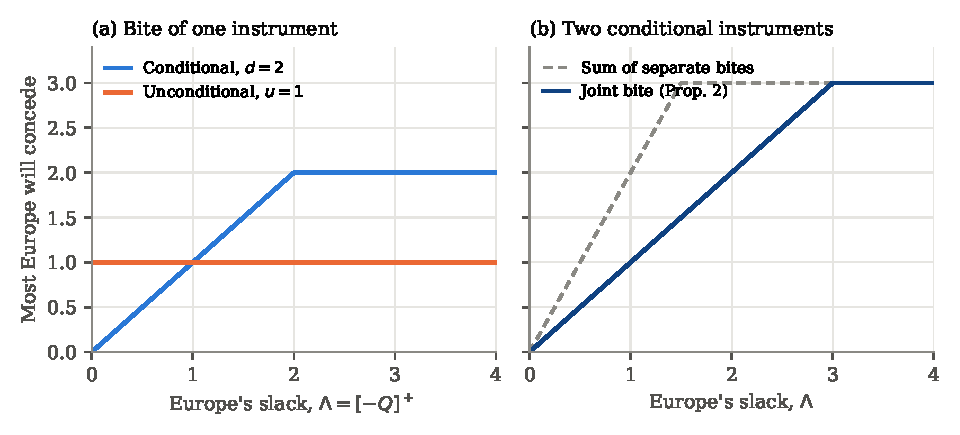
\includegraphics[width=0.95\textwidth]{figures/fig_slack.pdf}
\caption{The slack budget. Panel (a): the bite of a conditional instrument with $d=2$ rises one for one with Europe's slack $\Lambda$ until $\Lambda=2$; an unconditional instrument with $u=1$ bites the same at every $\Lambda$. Panel (b): two conditional instruments with $d=1.5$ each. The sum of their separate bites (dashed) overstates their joint bite $\min\{3,\Lambda\}$ at every $\Lambda<3$. Bites from \cref{prop:slack}(a).}
\label{fig:slack}
\end{figure}

In panel (a) of \cref{fig:slack} the unconditional threat is the smaller one, yet it is the only one that still works as $\Lambda$ falls toward zero. Panel (b) illustrates part (c)(i). A coercer that prices each conditional threat on its own counts the same slack twice: at $\Lambda=1$ the separate bites sum to $2$ and the joint bite is $1$.

The bound in (c)(i) holds because Europe can always refuse every ultimatum, and the worst that refusal brings is the withdrawal of a subset of $J^c$. It needs a fixed credible set: if a refusal could make a new instrument credible, Europe's loss could exceed the bite of the initial set. Under the stake technology of \cref{sec:commitment} an instrument is credible when its execution cost is at most $\bar m_U$, whatever has happened before, so the set does not move.

\paragraph{What is new here.} The participation constraint and its slack are \citeauthor{clayton2026putting}'s: ``Threats generate power to the extent that they generate slack in the participation constraint'' \citep{clayton2026putting}. In their framework the pooled threats are enforcement threats. They raise the target's inside option, and the hegemon charges for the surplus they create; threats to cut off a target that refuses appear only in the supplement (Section B.3.1) of \citet{clayton2026framework}, where they are partly self-defeating. Washington's instruments against Europe are cut-off threats aimed at an ally that a rival is bidding for. Taking them seriously yields three results. Only the conditional part of an instrument is capped by slack. Conditional bites are not additive, so instruments that deter the same exit compete for one budget. And a coercer that cannot commit to stop demanding obtains less (part (d)), because a threat that deters is not used up and will back the next demand. Europe concedes only if the total it expects to concede, counting what the unspent threat will extract later, stays within the bite; with $b+1$ identical sunk demands, a single ultimatum would obtain $b$ of them and the adaptive sequence obtains none. The problem is an old one in the theory of strategic moves \citep{schelling1960strategy}: a threat meant to induce compliance works only if the target believes that compliance will end it. Part (d) puts it in a form close to \citeauthor{pauly2024damned}'s assurance dilemma: steps that make a coercer's threats credible weaken its assurance that compliance ends the punishment \citep{pauly2024damned}. Washington can buy the commitment with a staked promise to make no further demand in the period, which is credible if $\bar m_U$ exceeds the value of further extraction.\footnote{Spent threats can also serve as a commitment device. Take two instruments with $u=1.2$ and $u=1.0$ ($d=0$), sunk demands with $t=1$ ($w=5$) and $t=1.5$ ($w=1$), and execution cost $0.1$ for each instrument. A single ultimatum yields $5$. In every subgame perfect equilibrium of the adaptive protocol, Washington first issues an ultimatum that Europe refuses, which burns one instrument, and then obtains the first demand, for a payoff of $4.9$.}

Washington's choice of demands follows from parts (b) to (d).

\begin{corollary}[Rationing]\label{cor:rationing}
Suppose all demands are reversible and either the United States can commit to a single ultimatum or $B(J^c)\ge\Lambda$. Then its optimal demand set solves
\[ \max_{y\in\{0,1\}^K}\ \sum_k w_k y_k-\pos{\textstyle\sum_k t_k y_k-\Lambda}
   \quad\text{s.t.}\quad \min\Big\{\sum_k t_k y_k,\Lambda\Big\}\le B(J^c). \]
This is the knapsack $\max\sum_k w_k y_k$ s.t.\ $\sum_k t_k y_k\le\min\{\Lambda,B(J^c)\}$ if $B(J^c)<\Lambda$, or if demands are divisible ($y\in[0,1]^K$) and $w_k\le t_k$ for every $k$. In general the United States may exceed $\Lambda$ and pay the excess back as rent. The free capacity $\min\{\Lambda,B(J^c)\}$ falls as $Q$ rises toward $0$. Demands from every issue area draw on it.
\end{corollary}

The corollary is a theory of how a patron rations coercion across its demands on an ally. Export-control alignment and limits on servicing in China are reversible concessions (\cref{sec:background}). So are the trade terms of August 2025, under which the EU said it would eliminate tariffs on US industrial goods and adopt technology-security requirements in line with those of the United States \citep{whitehouse2025jointstatement}. The NATO commitment to spend 5 percent of GDP on defence and related items by 2035 \citep{nato2025hague} and the EU's stated intention to increase procurement of US military equipment \citep{whitehouse2025jointstatement} are closer to sunk, since they cost Europe whatever it later does with ASML. A demand on Europe's digital rules would draw on the same budget. For Washington these demands are substitutes. The reversible ones share the capacity $\min\{\Lambda,B(J^c)\}$, so a concession extracted on tariffs leaves less to extract on servicing, and the sunk ones draw down the unconditional part of the bite. Washington links the issues openly. At The Hague in June 2025, Trump answered Spain's refusal of the spending target by saying ``We're negotiating with Spain on a trade deal. We're going to make them pay twice as much'' \citep{rte2025nato}. In the model this moves one budget between demands. The budget shrinks as China's credible offer rises, so a patron facing a holder whose premium approaches zero must drop demands, starting with those of lowest value per unit of European cost.

\subsection{Counter-threats and hedges}\label{sec:counter}

We do not let China punish alignment as such. Its coercion of US allies has been aimed at specific acts. When Washington pressed Tokyo in 2024 to restrict Tokyo Electron's sales and servicing in China, Beijing threatened ``severe economic retaliation'' \citep{taipeitimes2024retaliation}, and the first use of its new regulation on countering foreign extraterritorial jurisdiction was a May 2026 determination against the Commission's investigation of Nuctech under the Foreign Subsidies Regulation \citep{cleary2026nuctech}. We therefore model Chinese coercion as counter-threats attached to particular concessions, announced before Washington makes its demands. We also consider a hedge: legacy-tool sales and servicing worth $y_H$ to Europe and $w_H$ to Washington if stopped. Washington can stop the hedge in two ways. It can demand it as a concession backed by $J^c$ (linkage), or it can threaten to block the hedged flows with its jurisdiction over them, at net ex post cost $e_F$.

\begin{proposition}[Counter-threats and hedges]\label{prop:counter}
Maintain the assumptions of \cref{prop:slack}.
\begin{enumerate}[label=(\alph*)]
\item \emph{Counter-threats.} Before the United States moves, China chooses credible counter-threats $r_k\in[0,\bar r_k]$. If concession $k$ is made and $r_k>0$, China executes at cost $e^C_k>0$ and Europe bears the sunk loss $r_k$. China loses $z_k\ge 0$ when concession $k$ is made. The United States makes a single ultimatum backed by $J^c$, and its optimal bundle is unique at the profiles compared below.
  \begin{enumerate}[label=(\roman*)]
  \item A counter-threat adds $r_k$ to the sunk cost of $k$: Europe accepts $S$ if and only if
  \[ \min\{T_{\mathrm r}(S),\Lambda\}+T_{\mathrm s}(S)+\textstyle\sum_{k\in S}r_k\le B(J^c). \]
  \item China does better than with no threats only if the United States' demand set changes.
  \item If a counter-threat on $k$ is executed in China's optimal profile, then dropping it changes the United States' demand set to one that contains a demand outside the equilibrium set. China executes on path only to crowd out other demands, and this occurs for an open set of parameters.
  \item The United States' payoff is weakly lower under any profile of counter-threats.
  \item Europe's net loss is at most $B(J^c)$ with or without counter-threats. It equals $B(J^c)$ in both cases if the United States has a divisible sunk demand of positive value that China cannot threaten. The counter-threat then taxes the patron, not the holder. Otherwise Europe's loss can rise or fall.
  \end{enumerate}
\item \emph{Policing a hedge.} Stopping a hedge worth $y_H$ to Europe is a reversible concession. If it is the only demand, linkage stops the hedge if and only if $\min\{y_H,\Lambda\}\le B(J^c)$ and $w_H\ge\pos{y_H-\Lambda}$, where $w_H$ is its value to the United States. The United States then pays rent $\pos{y_H-\Lambda}$. Linkage is free only if $y_H\le\min\{\Lambda,B(J^c)\}$, and its free part $\min\{y_H,\Lambda\}$ vanishes as $Q\to 0$. A staked threat to block the hedge by flow jurisdiction, with net ex post cost $e_F$, is credible if and only if $e_F\le\bar m_U$. It leaves $Q$ unchanged and is never executed. Executing a conditional withdrawal $J$ raises Europe's premium to $Q+d(J)$.
\end{enumerate}
\end{proposition}

Part (a) changes who pays for Chinese coercion. A counter-threat makes a concession more expensive for Europe, and by (a)(i) it does so exactly as a sunk cost would. If Washington has other demands that China cannot reach, it fills the budget with them, and Europe's loss stays at $B(J^c)$. What changes is the mix. Washington gives up the demand China has made expensive and takes others it values less, so the counter-threat taxes the patron. China gains only by changing what Washington asks for (part (a)(ii)), and it carries out a threat only when doing so crowds out some other demand (part (a)(iii)). A numerical case shows that this can happen on the equilibrium path. Let $B(J^c)=2$. Demand 1 is sunk, with $t_1=0.3$, $w_1=1$ and $z_1=5$, and China cannot threaten it. Demand 2 is sunk, with $t_2=1.5$ and $w_2=20$, and China can attach $\bar r_2=0.4$ to it at execution cost $0.1$. Without counter-threats Washington asks for both. With $r_2=0.4$ the pair would cost Europe $2.2>2$, so Washington keeps the valuable demand 2 and drops demand 1, and China executes its threat. China's payoff rises from $-5$ to $-0.1$, and Europe's loss rises from $1.8$ to $1.9$. Under complete information, then, an executed Chinese counter-threat needs a demand it crowded out. \Cref{sec:record} reads the Nexperia episode with this requirement in mind; the alternative is that The Hague misjudged China's resolve, which lies outside this complete-information model.

Part (b) yields the prediction that separates the slack logic from simple cost minimization. A coercer that minimizes cost polices partial defection with whatever credible instrument is cheapest, and sizes sanctions so that punishing the small offence does not erode deterrence of the large one \citep{stigler1970optimum, shavell1992note}. Holding the costs of instruments fixed, that account predicts no change in Washington's choice of instrument as Europe's outside option improves. The slack principle predicts a change. The free part of linkage, $\min\{y_H,\Lambda\}$, shrinks as the premium rises toward zero, and beyond it Washington must pay the rent $\pos{y_H-\Lambda}$ to use linkage at all. Flow jurisdiction does not depend on slack: it is credible whenever $e_F\le\bar m_U$, it leaves $Q$ unchanged, and under complete information it deters without being used. So linkage against hedging should appear when the ally has slack and fade as its premium approaches zero, even where flow jurisdiction is unavailable, while the use of flow jurisdiction should not track the ally's premium at all. Linkage is also a wasting asset once used: a conditional withdrawal that is carried out raises Europe's premium by $d(J)$, so the instrument that punished the hedge no longer deters exit.

The record fits the first half of this prediction. The 2025 National Security Strategy ties favourable treatment to export-control alignment (\cref{sec:conditionality}), and in the August 2025 joint statement the United States undertook to facilitate exports of AI chips to the EU once the EU adopted technology-security requirements in line with its own \citep{whitehouse2025jointstatement}. Both tie the AI instrument and commercial instruments to export-control alignment, a reversible concession. That is what part (b) leads us to expect from a patron dealing with an ally that has slack. The second half, the retreat from linkage as the premium approaches zero, needs variation in premia that the Dutch record alone does not supply. \Cref{sec:tests} outlines a comparison across holders (the Netherlands, Japan and South Korea) and over time.

\subsection{Conditionality as a choice}\label{sec:conditionality}

So far conditionality has been a parameter. Washington chooses it. Recall from \cref{sec:security} that Washington defends Europe in a crisis if its stake in Europe's security exceeds a crisis cost $\xi$ drawn from a continuous distribution $G$ with density $g$, that its stake is $s_A=s_X+s_L$ in a loyal Europe and $s_X=s_0+s_B$ in one that has exited, and that a public stake $m_S\le\bar m_U$ on abandoning an exiter makes the core guarantee conditional by $\kappa=G(s_A)-G(s_X-m_S)$. Choosing $m_S$ is choosing $\kappa\in[\kappa_0,\bar\kappa]$, where $\kappa_0=G(s_A)-G(s_X)$ is the conditionality with no stake and $\bar\kappa=G(s_A)-G(s_X-\bar m_U)$ the largest Washington can create.

Conditionality is costly to the coercer, and we let it cost $H(\kappa)$, increasing and convex with $H(\kappa_0)=0$. The cost is one of assurance: other allies discount a guarantee that comes with a broad withdrawal rule, and a guarantee tied to Europe's conduct can be triggered by mistake. With $Q_0$ the premium at $\kappa_0$, the premium is $Q(\kappa)=Q_0-(\kappa-\kappa_0)S_k$. Washington converts slack into concessions worth $\nu\in[0,1]$ per unit of European cost; by \cref{cor:rationing}, $\nu$ is the value of its best reversible demands, and we assume $B(J^c)\ge\Lambda$ so that all slack can be converted. Washington chooses $\kappa$ before the bidding stage to maximize
\[
\Pi(\kappa)=-\pos{Q(\kappa)}+\nu\,\pos{-Q(\kappa)}-H(\kappa).
\]
Let $H'$ be the right derivative of $H$. For $x\ge 0$ let $\kappa_x=\inf\{\kappa\in[\kappa_0,\bar\kappa]:H'(\kappa)\ge x\}$, with $\inf\emptyset=+\infty$, and write $\kappa_1=\kappa_{S_k}$ and $\kappa_\nu=\kappa_{\nu S_k}$, so that $\kappa_0\le\kappa_\nu\le\kappa_1$. The conditionality at which the premium is exactly zero is $\kappa_z=\kappa_0+Q_0/S_k$.

\begin{proposition}[Conditionality is the price of concessions]\label{prop:conditionality}
The conditionality
\[ \kappa^*=\min\big\{\bar\kappa,\ \max\{\kappa_\nu,\ \min\{\kappa_z,\kappa_1\}\}\big\} \]
maximizes $\Pi$, uniquely if $H$ is strictly convex, and $Q(\kappa^*)=(\kappa_z-\kappa^*)S_k$.
\begin{enumerate}[label=(\alph*)]
\item If $\nu=0$, then $\kappa^*=\kappa_0$ when $Q_0\le 0$, and $\kappa^*=\min\{\kappa_z,\kappa_1,\bar\kappa\}$ otherwise. The United States never makes its guarantee more conditional than needed to hold the premium at zero. It creates no slack: $\Lambda^*=\pos{-Q_0}$.
\item If $\nu>0$, $\kappa_0\le\kappa_z<\bar\kappa$ and $H'(\kappa_z)<\nu S_k$, then $\kappa^*=\min\{\kappa_\nu,\bar\kappa\}>\kappa_z$ and $\Lambda^*=(\kappa^*-\kappa_z)S_k>0$: conditionality is the price of concessions. If $Q_0<0$, then $\kappa^*=\min\{\kappa_\nu,\bar\kappa\}$ and $\Lambda^*=(\kappa^*-\kappa_z)S_k\ge -Q_0$.
\item Let $H$ be strictly convex and differentiable. Away from regime boundaries:
  \begin{enumerate}[label=(\roman*)]
  \item if $\kappa^*=\kappa_z$, then $d\kappa^*/dQ_0=1/S_k$ and the United States pays no rent: a stronger Chinese bid elicits a more conditional guarantee, not a payment;
  \item if $\kappa^*=\kappa_1<\min\{\kappa_z,\bar\kappa\}$ (assurance is costly at the margin before the premium reaches zero), $\kappa^*$ does not depend on $Q_0$ and the rent $Q(\kappa_1)>0$ rises one for one with $Q_0$;
  \item if $\kappa^*=\kappa_\nu\in(\max\{\kappa_z,\kappa_0\},\bar\kappa)$, or if $\kappa^*=\kappa_0>\kappa_z$, then $\kappa^*$ does not depend on $Q_0$ and slack falls one for one with $Q_0$: China's bid is paid for out of the United States' concessions;
  \item if $\kappa^*=\bar\kappa$, the United States pays $\pos{Q(\bar\kappa)}$, which rises one for one with $Q_0$ when $Q(\bar\kappa)>0$. Otherwise slack falls one for one.
  \end{enumerate}
\item $d\bar\kappa/ds_X=g(s_X+s_L)-g(s_X-\bar m_U)$, with $s_L$ and $\bar m_U$ fixed. Hence $\bar\kappa$ is nonincreasing in $s_X$ wherever $g$ is nonincreasing on $[s_X-\bar m_U,\,s_X+s_L]$, for example when Washington would almost surely defend a loyal Europe, and it is then nonincreasing in the access value of European territory and, if $s_B$ rises with $V$, in $V$. If instead $g(s_X+s_L)>g(s_X-\bar m_U)$, $\bar\kappa$ rises with $s_X$. If $s_A$ is held fixed when $s_X$ rises, $\bar\kappa$ is nonincreasing in $s_X$ for every $G$.
\end{enumerate}
\end{proposition}

If conditionality cost nothing, Washington would set it at $\bar\kappa$. With an assurance cost, how conditional the guarantee is depends on what Washington wants from Europe. A patron with no further demands ($\nu=0$) makes its guarantee just conditional enough to hold the premium at zero, or less if assurance becomes too costly first, and it creates no slack. Conditionality beyond that point is worth buying only because slack can be spent, so the patron that plans to make demands is the one that makes its guarantee more conditional than the rivalry with China requires. That is the sense in which conditionality is the price of concessions: Europe pays for the extra conditionality with the concessions it then makes, and other allies pay through a weaker assurance. The argument uses only the fact that Washington chooses a conditional part before the bidding stage at a convex cost, so it applies with $d_j$ in place of $\kappa S_k$ to any instrument whose conditional part Washington sets.

Part (c)(i) describes how a patron answers a stronger rival. In the bidding benchmark a rise in China's credible offer raises what Washington must pay once the premium is positive. When assurance is cheap at the margin, Washington instead makes its guarantee more conditional, by exactly enough to keep the premium at zero, and pays nothing. The December 2025 National Security Strategy reads this way to us. It promises ``more favorable treatment on commercial matters, technology sharing, and defense procurement'' to countries that ``align their export controls with ours'' \citep{whitehouse2025nss}. The passage makes treatment depend on alignment, which raises conditional parts relative to the treatment of a country that does not align. In the model's terms this is conditionality. A transfer would be provision above the aligned baseline, which is due only when the premium is positive. \Cref{sec:coding} sets out how we code the two in the record. Where assurance is already costly at the margin, or Washington is already spending slack, parts (c)(ii) and (c)(iii) say who pays for China's bid instead: Washington in rent, or Washington in forgone concessions.

Two kinds of US drawdown have opposite places in the model. An untargeted drawdown lowers what Washington provides to a loyal ally, $x_p(A)$, and so lowers the conditional part $d_p$ of posture and enablers along with Europe's slack. The withdrawal of 25,000 or more troops from Europe that the Pentagon was reported in September 2026 to be weighing \citep{nbc2026pentagon} would be a cut of this kind, to the extent that it is not aimed at particular allies' conduct. A targeted withdrawal after defiance is different. The order of 1 May 2026 to move about 5,000 troops out of Germany followed Chancellor Merz's criticism of US strategy on Iran \citep{martinez2026germany} (see \cref{sec:background}). It punished an act, so in the model it is an executed threat, and \cref{prop:counter}(b) says what execution does: it spends the instrument and raises the target's premium by the instrument's conditional part, since posture already withdrawn cannot be withheld again. Whether the order also raised other allies' beliefs about how conditional US protection is depends on reputation and on uncertainty about $\kappa$, which this complete-information model leaves out.

Part (d) gives the sign of the silicon shield, the fourth channel of \cref{cor:master}. If holding the chokepoint raises Washington's own stake in Europe's security whatever Europe's alignment, then $s_X$ rises. In the case the proposition singles out, where Washington would almost surely defend a loyal Europe, the higher $s_X$ lowers the most conditionality Washington can create. The chokepoint then limits how far its holder can be coerced through the guarantee. The same comparative static holds for the access value of European territory, which also raises $s_X$ \citep{carson2025allies}. Where defence of a loyal Europe is in real doubt, the sign can reverse, and holding the chokepoint can make the guarantee more conditional. Part (d) therefore makes the silicon shield an empirical question about the distribution of crisis costs.

The assurance literature supplies the cost side of the proposition. \citet{pauly2024damned} shows that the steps a coercer takes to make a threat credible undermine its assurance that compliance will not be punished. In our model those steps are the stakes that raise $\kappa$, and part of their cost is $H$. \citet{gerzhoy2015alliance} credits US abandonment threats, paired with that kind of assurance, with restraining West Germany; \citet{lanoszka2018atomic} disputes that they were decisive and finds that allies who doubt the patron build capabilities of their own. Such capabilities raise the ally's premium, as Europe's autonomy investment does in \cref{sec:control}, and the prospect of them is a second component of $H$. \citet{blankenship2021price} finds that US pressure on allies works when Washington can credibly threaten to reduce protection, and that allies in locations the United States values contribute less. That pattern is what part (d) implies when the density of crisis costs is decreasing: a higher $s_X$ lowers the conditionality Washington can credibly create.
